%%%%%%%%%%%%%%%%%%%%%%%%%%%%%%%%%%%%%%%%%
% Programming/Coding Assignment
% LaTeX Template
%
% This template has been downloaded from:
% http://www.latextemplates.com
%
% Original author:
% Ted Pavlic (http://www.tedpavlic.com)
%
% Note:
% The \lipsum[#] commands throughout this template generate dummy text
% to fill the template out. These commands should all be removed when 
% writing assignment content.
%
% This template uses a Perl script as an example snippet of code, most other
% languages are also usable. Configure them in the "CODE INCLUSION 
% CONFIGURATION" section.
%
%%%%%%%%%%%%%%%%%%%%%%%%%%%%%%%%%%%%%%%%%

%----------------------------------------------------------------------------------------
%	PACKAGES AND OTHER DOCUMENT CONFIGURATIONS
%----------------------------------------------------------------------------------------

\documentclass{article}

\usepackage{fancyhdr} % Required for custom headers
\usepackage{lastpage} % Required to determine the last page for the footer
\usepackage{extramarks} % Required for headers and footers
\usepackage[usenames,dvipsnames]{color} % Required for custom colors
\usepackage{graphicx} % Required to insert images
\usepackage{subcaption}
\usepackage{listings} % Required for insertion of code
\usepackage{courier} % Required for the courier font
\usepackage{lipsum} % Used for inserting dummy 'Lorem ipsum' text into the template
\usepackage{listings}
\usepackage{amsmath}

% Margins
\topmargin=-0.45in
\evensidemargin=0in
\oddsidemargin=0in
\textwidth=6.5in
\textheight=9.0in
\headsep=0.25in

\linespread{1.1} % Line spacing

% Set up the header and footer
\pagestyle{fancy}
\lhead{\hmwkAuthorName} % Top left header
%\chead{\hmwkClass\ (\hmwkClassTime): \hmwkTitle} % Top center head
%\rhead{\firstxmark} % Top right header
\lfoot{\lastxmark} % Bottom left footer
\cfoot{} % Bottom center footer
\rfoot{Page\ \thepage\ of\ \protect\pageref{LastPage}} % Bottom right footer
\renewcommand\headrulewidth{0.4pt} % Size of the header rule
\renewcommand\footrulewidth{0.4pt} % Size of the footer rule

\setlength\parindent{0pt} % Removes all indentation from paragraphs

%----------------------------------------------------------------------------------------
%	CODE INCLUSION CONFIGURATION
%----------------------------------------------------------------------------------------

\definecolor{MyDarkGreen}{rgb}{0.0,0.4,0.0} % This is the color used for comments
\lstloadlanguages{Perl} % Load Perl syntax for listings, for a list of other languages supported see: ftp://ftp.tex.ac.uk/tex-archive/macros/latex/contrib/listings/listings.pdf
\lstset{language=Perl, % Use Perl in this example
        frame=single, % Single frame around code
        basicstyle=\small\ttfamily, % Use small true type font
        keywordstyle=[1]\color{Blue}\bf, % Perl functions bold and blue
        keywordstyle=[2]\color{Purple}, % Perl function arguments purple
        keywordstyle=[3]\color{Blue}\underbar, % Custom functions underlined and blue
        identifierstyle=, % Nothing special about identifiers                                         
        commentstyle=\usefont{T1}{pcr}{m}{sl}\color{MyDarkGreen}\small, % Comments small dark green courier font
        stringstyle=\color{Purple}, % Strings are purple
        showstringspaces=false, % Don't put marks in string spaces
        tabsize=5, % 5 spaces per tab
        %
        % Put standard Perl functions not included in the default language here
        morekeywords={rand},
        %
        % Put Perl function parameters here
        morekeywords=[2]{on, off, interp},
        %
        % Put user defined functions here
        morekeywords=[3]{test},
       	%
        morecomment=[l][\color{Blue}]{...}, % Line continuation (...) like blue comment
        numbers=left, % Line numbers on left
        firstnumber=1, % Line numbers start with line 1
        numberstyle=\tiny\color{Blue}, % Line numbers are blue and small
        stepnumber=5 % Line numbers go in steps of 5
}

% Creates a new command to include a perl script, the first parameter is the filename of the script (without .pl), the second parameter is the caption
\newcommand{\perlscript}[2]{
\begin{itemize}
\item[]\lstinputlisting[caption=#2,label=#1]{#1.pl}
\end{itemize}
}

%----------------------------------------------------------------------------------------
%	DOCUMENT STRUCTURE COMMANDS
%	Skip this unless you know what you're doing
%----------------------------------------------------------------------------------------

% Header and footer for when a page split occurs within a problem environment
\newcommand{\enterProblemHeader}[1]{
%\nobreak\extramarks{#1}{#1 continued on next page\ldots}\nobreak
%\nobreak\extramarks{#1 (continued)}{#1 continued on next page\ldots}\nobreak
}

% Header and footer for when a page split occurs between problem environments
\newcommand{\exitProblemHeader}[1]{
%\nobreak\extramarks{#1 (continued)}{#1 continued on next page\ldots}\nobreak
%\nobreak\extramarks{#1}{}\nobreak
}

\setcounter{secnumdepth}{0} % Removes default section numbers
\newcounter{homeworkProblemCounter} % Creates a counter to keep track of the number of problems
\setcounter{homeworkProblemCounter}{-1}

\newcommand{\homeworkProblemName}{}
\newenvironment{homeworkProblem}[1][Problem \arabic{homeworkProblemCounter}]{ % Makes a new environment called homeworkProblem which takes 1 argument (custom name) but the default is "Problem #"
\stepcounter{homeworkProblemCounter} % Increase counter for number of problems
\renewcommand{\homeworkProblemName}{#1} % Assign \homeworkProblemName the name of the problem
\section{\homeworkProblemName} % Make a section in the document with the custom problem count
\enterProblemHeader{\homeworkProblemName} % Header and footer within the environment
}{
\exitProblemHeader{\homeworkProblemName} % Header and footer after the environment
}

\newcommand{\problemAnswer}[1]{ % Defines the problem answer command with the content as the only argument
\noindent\framebox[\columnwidth][c]{\begin{minipage}{0.98\columnwidth}#1\end{minipage}} % Makes the box around the problem answer and puts the content inside
}

\newcommand{\homeworkSectionName}{}
\newenvironment{homeworkSection}[1]{ % New environment for sections within homework problems, takes 1 argument - the name of the section
\renewcommand{\homeworkSectionName}{#1} % Assign \homeworkSectionName to the name of the section from the environment argument
\subsection{\homeworkSectionName} % Make a subsection with the custom name of the subsection
\enterProblemHeader{\homeworkProblemName\ [\homeworkSectionName]} % Header and footer within the environment
}{
\enterProblemHeader{\homeworkProblemName} % Header and footer after the environment
}

%----------------------------------------------------------------------------------------
%	NAME AND CLASS SECTION
%----------------------------------------------------------------------------------------

\newcommand{\hmwkTitle}{Final Project} % Assignment title
%\newcommand{\hmwkDueDate}{YYY,\ 2019} % Due date
\newcommand{\hmwkClass}{MAT4373} % Course/class
%\newcommand{\hmwkClassTime}{L0101} % Class/lecture time
\newcommand{\hmwkAuthorName}{Team Cool} % Your name

%----------------------------------------------------------------------------------------
%	TITLE PAGE
%----------------------------------------------------------------------------------------

\title{
\vspace{2in}
\textmd{\textbf{\hmwkClass:\ \hmwkTitle}}\\[5pt]
\normalsize{Part 1: Option B}\\
\vspace{0.1in}
\vspace{3in}
}

%\author{}


%----------------------------------------------------------------------------------------

\begin{document}

\maketitle
\begin{center}
\hmwkAuthorName\\[3pt]
\begin{tabular}{ll}
Anshu Sharma & 300011600 \\
Bhavika Sewpal & 300089940 \\
\end{tabular} 
\end{center}
\clearpage
%----------------------------------------------------------------------------------------
%	PROBLEM 0
%----------------------------------------------------------------------------------------

% To have just one problem per page, simply put a \clearpage after each problem
%For this project, you will build and train two systems for digit classification: one neural
%network and one linear classifier. Note: for the classifiers and settings suggested in this
%project, overfitting is not a significant problem; we therefore forego requiring that you
%have a validation set. You can nevertheless use one at your discretion.

\begin{homeworkProblem}

\noindent \textit{Project description}
We will be building two systems for digit classification. The first system is a linear classifier written from low level python library and the second system will be a neural network using the Keras library. We investigate how these model operate by graphing the model's loss function and accuracy rate, as well as generating heat maps with the models.\\

\noindent \textit{Dataset description}
We will be working with the MNSIT dataset for this project. The dataset consists of 70,000 grey-scale images of handwritten numerals. The each image is 28x28 image with the hand-written numeral centered in the image with variation on the hand writing. We split the dataset to 60,000 training and 10,000 testing images.\\

% \noindent \textit{Environment description}
% We ran our code in Google colab. To reproduce the results we obtained in our notebook, create a folder named MAT4373 in your google drive. Put the mnist_all.mat file inside the MAT4373 folder and run the notebook in google colab.
% Alternatively, if you want to run the code on your local computer, change the path in the code below to the path containing the mnist_all.mat file on your local computer.

\noindent \textit{Environment description}
We ran our code in Google Colab. To reproduce the results we obtained in our notebook, create a folder named MAT4373 in your google drive folder. Put the mnist\_all.mat file inside the MAT4373 folder and upload and run the notebook in Google colab.
Alternatively, if you want to run the code on your local computer, change the path in the code below to the path containing the mnist\_all.mat file on your local computer.
\begin{lstlisting}[language=Python]
    M = sio.loadmat("/content/drive/MyDrive/MAT4373/mnist_all.mat")
\end{lstlisting}



\end{homeworkProblem}
\clearpage
%----------------------------------------------------------------------------------------
%	PROBLEM 1
%----------------------------------------------------------------------------------------

\begin{homeworkProblem}
In this section, we plot 10 images of each digits from the training dataset.

\begin{figure*}[h!]
    \centering
    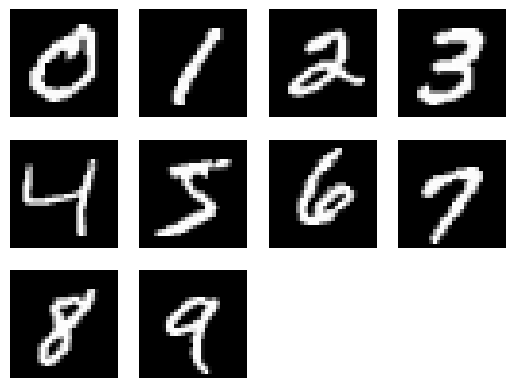
\includegraphics[scale=0.5]{MNISTsample.png}
    \caption{A selection of 10 images of each digits.}
    \label{fig:randim}
\end{figure*}

\end{homeworkProblem}
\clearpage
%----------------------------------------------------------------------------------------
%	PROBLEM 2
%----------------------------------------------------------------------------------------

\begin{homeworkProblem}
In this section, we implement a function that computes the network below. The o's here are simply the linear combinations of the x's. In our implementation, x is a vector of size 785, which is obtained by flattening the 28x28 image and adding a first entry equal to 1 to account for the input to the bias.

\begin{figure*}[h!]
    \centering
    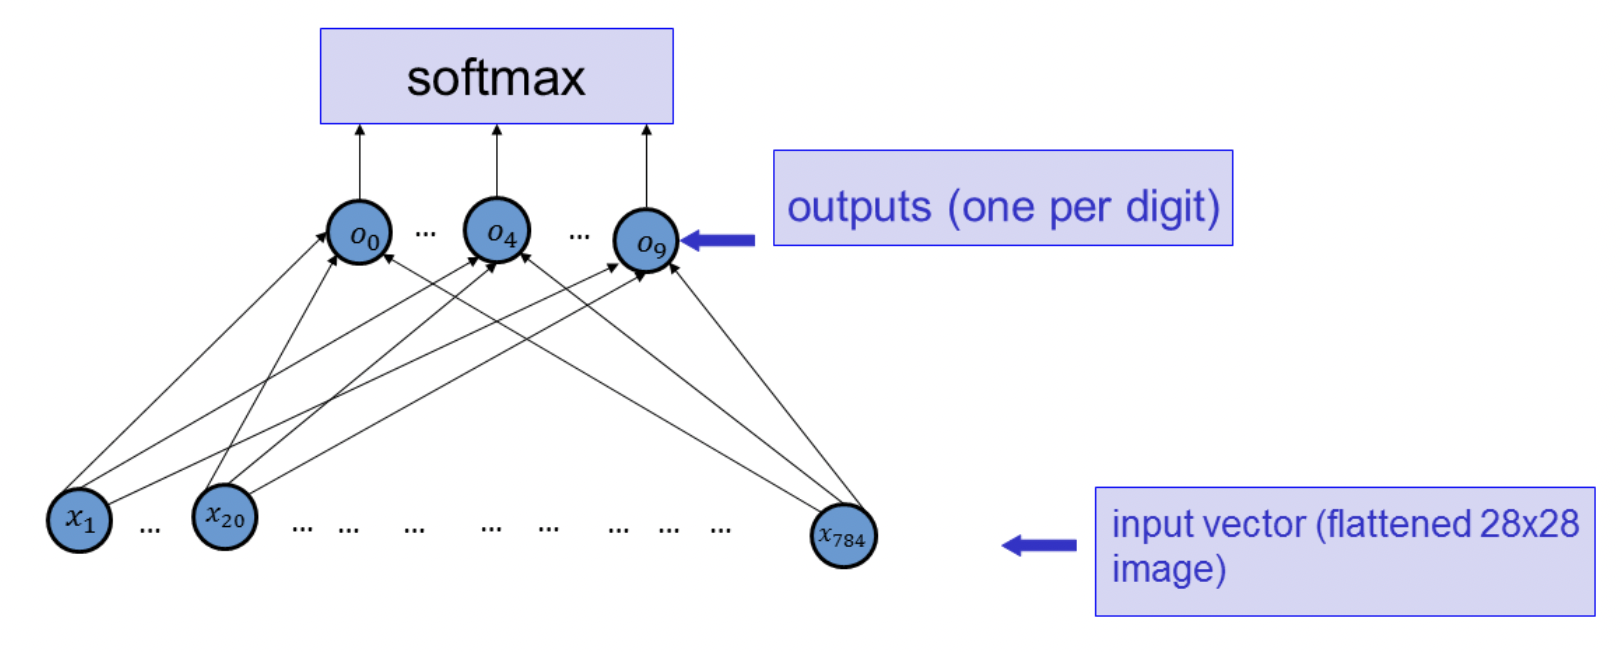
\includegraphics[scale=0.5]{network_from_scratch.png}
    \caption{Diagram for the neural network implemented from scratch.}
    \label{fig:randim}
\end{figure*}

\begin{align*}
    & o_i = \sum_{j=1}^{785}w_{ji}x_j,\hspace{0.5 cm} 0 \leq i \leq 9 \\
    & \hat{y_i} = \frac{e^{o_i}}{\sum_{i=0}^{9}e^{o_i}} \\
\end{align*}
The probability of an image belonging to any particular class i (where i ranges from 0 to 9) is given by the softmax equation above.
\begin{lstlisting}[language=Python]
class Layer_Dense:
    def __init__(self, n_inputs=784, n_neurons=10):
        self.weights = 0.10 * np.random.randn(n_inputs, n_neurons)
        # set bias to 0
        self.weights = np.insert(self.weights, 0,0, axis=0)

    def forward(self, inputs):
        self.output = np.dot(inputs, self.weights)
        
class Activation_Softmax:
    def forward(self, inputs):
        exp_values = np.exp(inputs - np.max(inputs, axis=1, keepdims=True))
        probabilities = exp_values / np.sum(exp_values, axis=1, keepdims=True)
        self.output = probabilities
\end{lstlisting}

The weights attribute in the Layer Dense class is a 785x10 matrix.
The output, i.e the logits of the neural network, is calculated by doing the dot product of the input (i.e the vector x of size 785) and the weights, according to the equation above.






\end{homeworkProblem}
\clearpage

%----------------------------------------------------------------------------------------
%	PROBLEM 3
%----------------------------------------------------------------------------------------

\begin{homeworkProblem}
For this network, we use the negative log loss function (also known as the cross-entropy loss function). A loss function is a function that compares the target and predicted output values. It measures how well the neural network models the training data. When training, we aim to minimize this loss between the predicted and target outputs. Each training input is loaded into the neural network in a process called forward propagation. Once the model has produced an output, this predicted output is compared against the given target output in a process called backpropagation. To do backpropagation, we need to find the derivative of the loss with respect to every single weight in the neural network (we have a total of 7850 weights in total).

Log loss function:
\begin{align*}
    &  L = - \sum_{i=0}^{9}y_i \log \hat{y_i}
\end{align*}
In the above formula, $\hat{y_i}$ is the probability computed for a given class by the neural network while  $y_i$ is the true value for that given class. $y_i$ are one-hot encoded in our implementation (i.e $y_i$ can either be 0 or 1). \\

The softmax function is defined as follows:
\begin{align*}
    & \hat{y_i} = \frac{e^{o_i}}{\sum_{k=0}^{9}e^{o_k}} \\
\end{align*} 

The logits (i.e $o_i$) are computed as follows:
\begin{align*}
    & o_i = \sum_{j=1}^{785}w_{ji}x_j
\end{align*} 

We now take the derivative of the loss wrt $\hat{y_i}$:
\begin{align*}
    \frac{\partial L}{\partial \hat{y_i}} = - \sum_{i=0}^{9}y_i \frac{1}{\hat{y_i}}
\end{align*} 

Let's take the derivative of $\hat{y_i}$ wrt $o_j$. \\
Let's consider the case where i = j:
\begin{align*}
    \frac{\partial \hat{y_i} }{\partial o_j} &= \frac{e^{o_j} \sum_{k=0}^{9}e^{o_k} - e^{o_j}e^{o_j} }{(\sum_{k=0}^{9}e^{o_k})^2} \\
    &= \frac{e^{o_j}}{\sum_{k=0}^{9}e^{o_k}} + 1 -  \frac{e^{o_j}}{\sum_{k=0}^{9}e^{o_k}}\\
    &= \hat{y_j}(1-\hat{y_j})
\end{align*} 

Let's consider the case where i $\neq$ j:
\begin{align*}
    \frac{\partial \hat{y_i} }{\partial \hat{o_j}} &= \frac{0 - e^{o_i}e^{o_j} }{(\sum_{k=0}^{9}e^{o_k})^2} \\
    &= -\hat{y_i}(\hat{y_j})
\end{align*} 

Let's now find the derivative of the loss L wrt to $o_i$. To do so, we use the chain rule.
\begin{align*}
    \frac{\partial L }{\partial \hat{o_j}} &= \frac{\partial L }{\partial \hat{y_i}} \frac{\partial \hat{y_i} }{\partial \hat{o_j}} \\
     &= -\sum_{i=0, i \neq j}^{9} \frac{y_i}{\hat{y_i}} (-\hat{y_i}\hat{y_j}) - \frac{y_j}{\hat{y_j}} (\hat{y_j}(1-\hat{y_j})) \\
     &= \sum_{i=0, i \neq j}^{9} {y_i}{\hat{y_j}} - y_j(1-\hat{y_j}) \\
     &= (\sum_{i=0, i \neq j}^{9} {y_i}{\hat{y_j}} + y_j\hat{y_j}) + y_j \\
     &= \sum_{j=0}^{9} {y_j}{\hat{y_j}} + y_j \\
     & = \hat{y_j} - y_j\\
\end{align*} 

Note: $\sum_{j=0}^{9} y_j = 1 $ since y is a one-hot encoded vector. For example, if an image belongs to class 0, its y vector will be [1 0 0 0 0 0 0 0 0 0]. \\

Finally, to find the derivative of the loss L wrt any weight in the model, we apply the chain rule again:

\begin{align*}
   \frac{\partial L }{\partial w_{ji}} &= \frac{\partial L }{\partial \hat{o_i}} \frac{\partial \hat{o_i} }{\partial {w_{ji}}} \\
   &= (\hat{y_i} - y_i)x_j \\
\end{align*} 

\begin{lstlisting}[language=Python]
    def calculate_derivatives(probabilities,input,target):
    batch_size = input.shape[0]
    input_size = 785
    output_size = 10
    
    derivatives = np.zeros(shape=(batch_size,input_size,output_size))
    diff = probabilities - target
    for i in range(batch_size):
    # current_diff contains 10 outputs for each 10 neurons
    current_diff = diff[i]
    # current_input contains 785 entries
    current_input = input[i]
    for j in range(input_size):
      input_entry = current_input[j]
      derivative = input_entry * current_diff
      derivatives[i][j] = derivative
    
    avg_derivative = np.mean(derivatives,axis=0)
    weight_updates = np.count_nonzero(avg_derivative)
    return avg_derivative, weight_updates
\end{lstlisting}










\end{homeworkProblem}
\clearpage 

%----------------------------------------------------------------------------------------
%	PROBLEM 4
%----------------------------------------------------------------------------------------

\begin{homeworkProblem}
In this section, we verify that we are computing the gradient in Part 3 correctly by computing it both using our function and using a finite-difference approximation.
Using the function below, we add a very small value h to the non-zero values in the training data.
\begin{lstlisting}
def add_diff(training_data, h=0.001):
  data = np.empty((training_data.shape[0],training_data.shape[1]))
  training_data = training_data.astype('float32') 
  for index ,element in enumerate(training_data):
    for i in range(len(element)):
      if element[i] != 0:
        element[i] = element[i]  + h
    data[index] = element
  return data
\end{lstlisting}

We then randomly initialise a layer. We do a forward and backward pass with a batch of the training data. We get the derivatives d of the weights and the new weights w1. We then add a small value h to the non-zero values in the batch and do a forward and backward pass with the batch. We get the new weights w2. If $\frac{w2 - w1}{h} = d$, we can be sure that our function is implementing back propagation properly.
\begin{lstlisting}
def finite_diff(training_data, training_target,layer, h =0.001):
  def calculate_weight(training_data, training_target,layer):
    activation = Activation_Softmax()
    layer.forward(training_data)
    logits = layer.output
    activation.forward(logits)
    probabilities = activation.output
    derivative,_ = calculate_derivatives(
        probabilities, training_data, encode(training_target))
    new_weights = adjust_weights(derivative,layer.weights)
    return new_weights, derivative

  weights,derivative = calculate_weight(training_data, training_target, layer)
  new_weights,_ = calculate_weight(
      add_diff(training_data , 0.001), training_target, layer)
  approximation = (new_weights - weights)/ (h * -0.01) # learning rate = -0.01

  return approximation, derivative
\end{lstlisting}

\begin{lstlisting}
layer = Layer_Dense()
approximation, derivative = finite_diff(
    training_data_bias_added[0:50],training_target[0:50],layer)
\end{lstlisting}

\clearpage
We then compared the derivative and its approximation with the function isclose from the numpy package. The following results were obtained:

\begin{figure*}[h!]
    \centering
    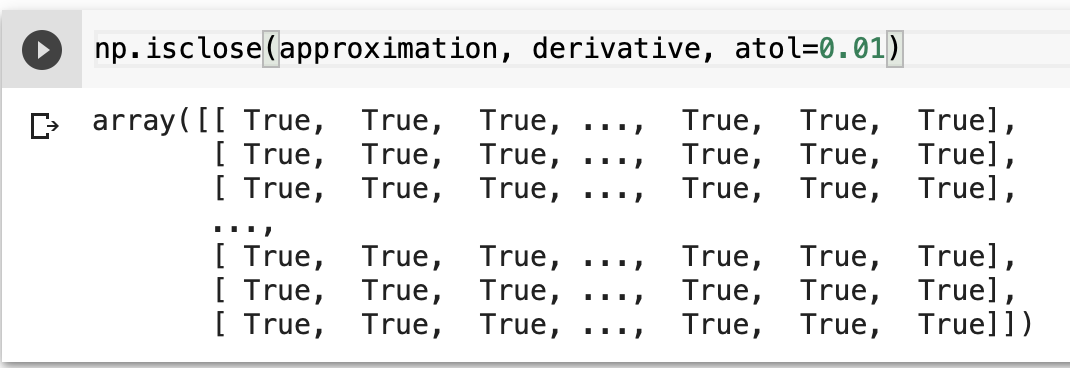
\includegraphics[scale=0.5]{isclose.png}
    \caption{Comparing the derivative and its approximation.}
    \label{fig:randim}
\end{figure*}


\end{homeworkProblem}
\clearpage


%----------------------------------------------------------------------------------------
%	PROBLEM 5
%----------------------------------------------------------------------------------------
\begin{homeworkProblem}
In this section, we train the neural network using mini-batch gradient descent. The batch size is equal to 50 and the learning rate is equal to 0.01. When doing backpropagation with batches, we calculate the derivative of the loss wrt to the weights for every image in the batch. We then compute the average and update the weights in the neural network according to this mean value. When using mini-batch gradient descent, the update frequency for the weights is higher than batch gradient descent. This allows for a more robust convergence, avoiding local minima.

Here are the pictures of 20 digits that were correctly classified:
\begin{figure*}[h!]
    \centering
    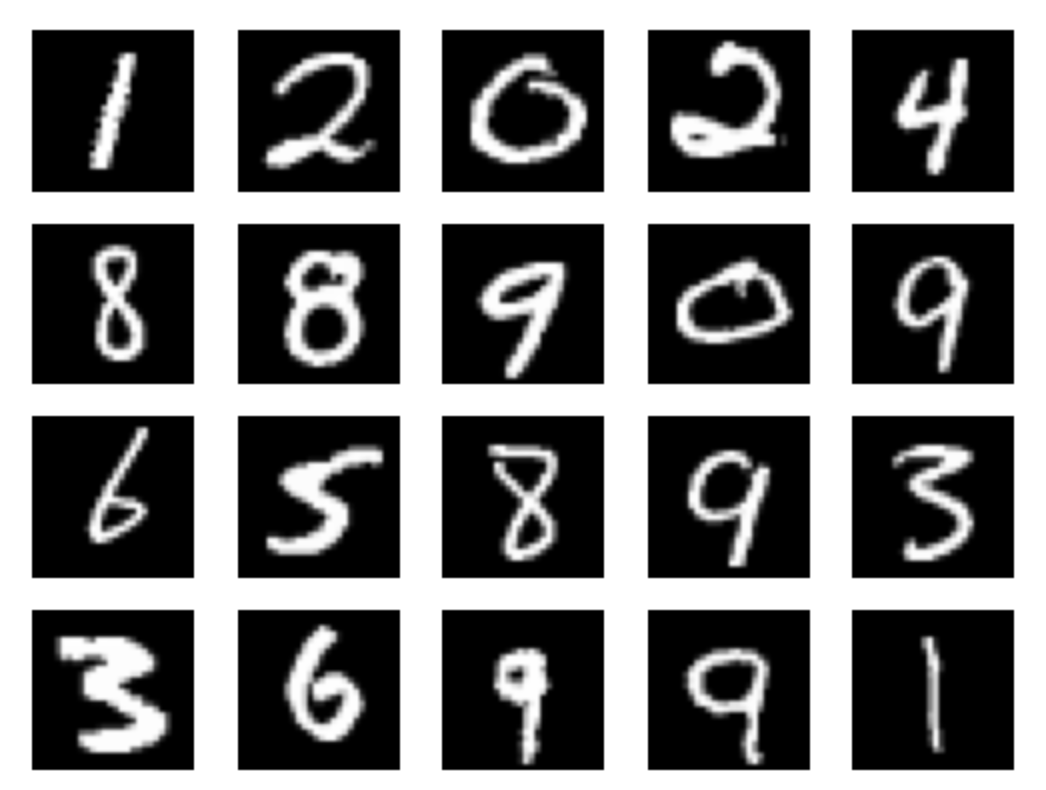
\includegraphics[scale=0.5]{correct.png}
    \caption{20 images that were correctly classified.}
    \label{fig:randim}
\end{figure*}

Here are the pictures of 10 digits that were incorrectly classified:
\begin{figure*}[h!]
    \centering
    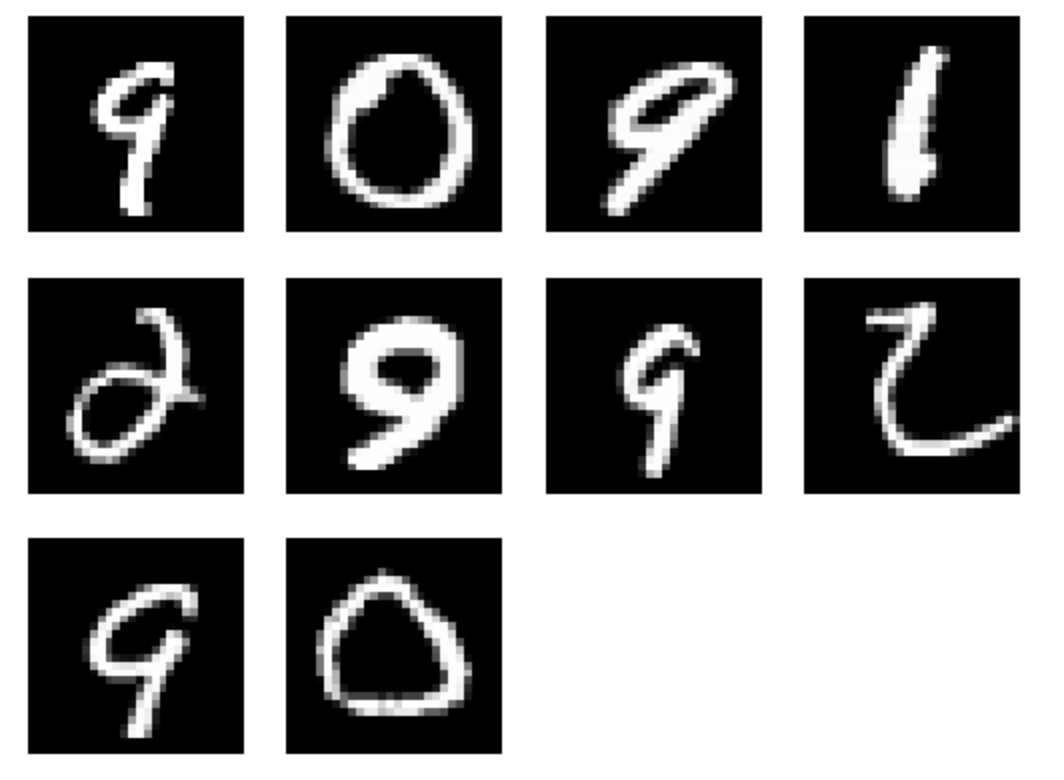
\includegraphics[scale=0.5]{incorrect.png}
    \caption{10 images that were correctly classified.}
    \label{fig:randim}
\end{figure*}

The model erroneously classified these pictures as 8, 8, 4, 8, 3, 8, 8, 5, 4 and 3. \\

\begin{figure*}[h!]
    \centering
    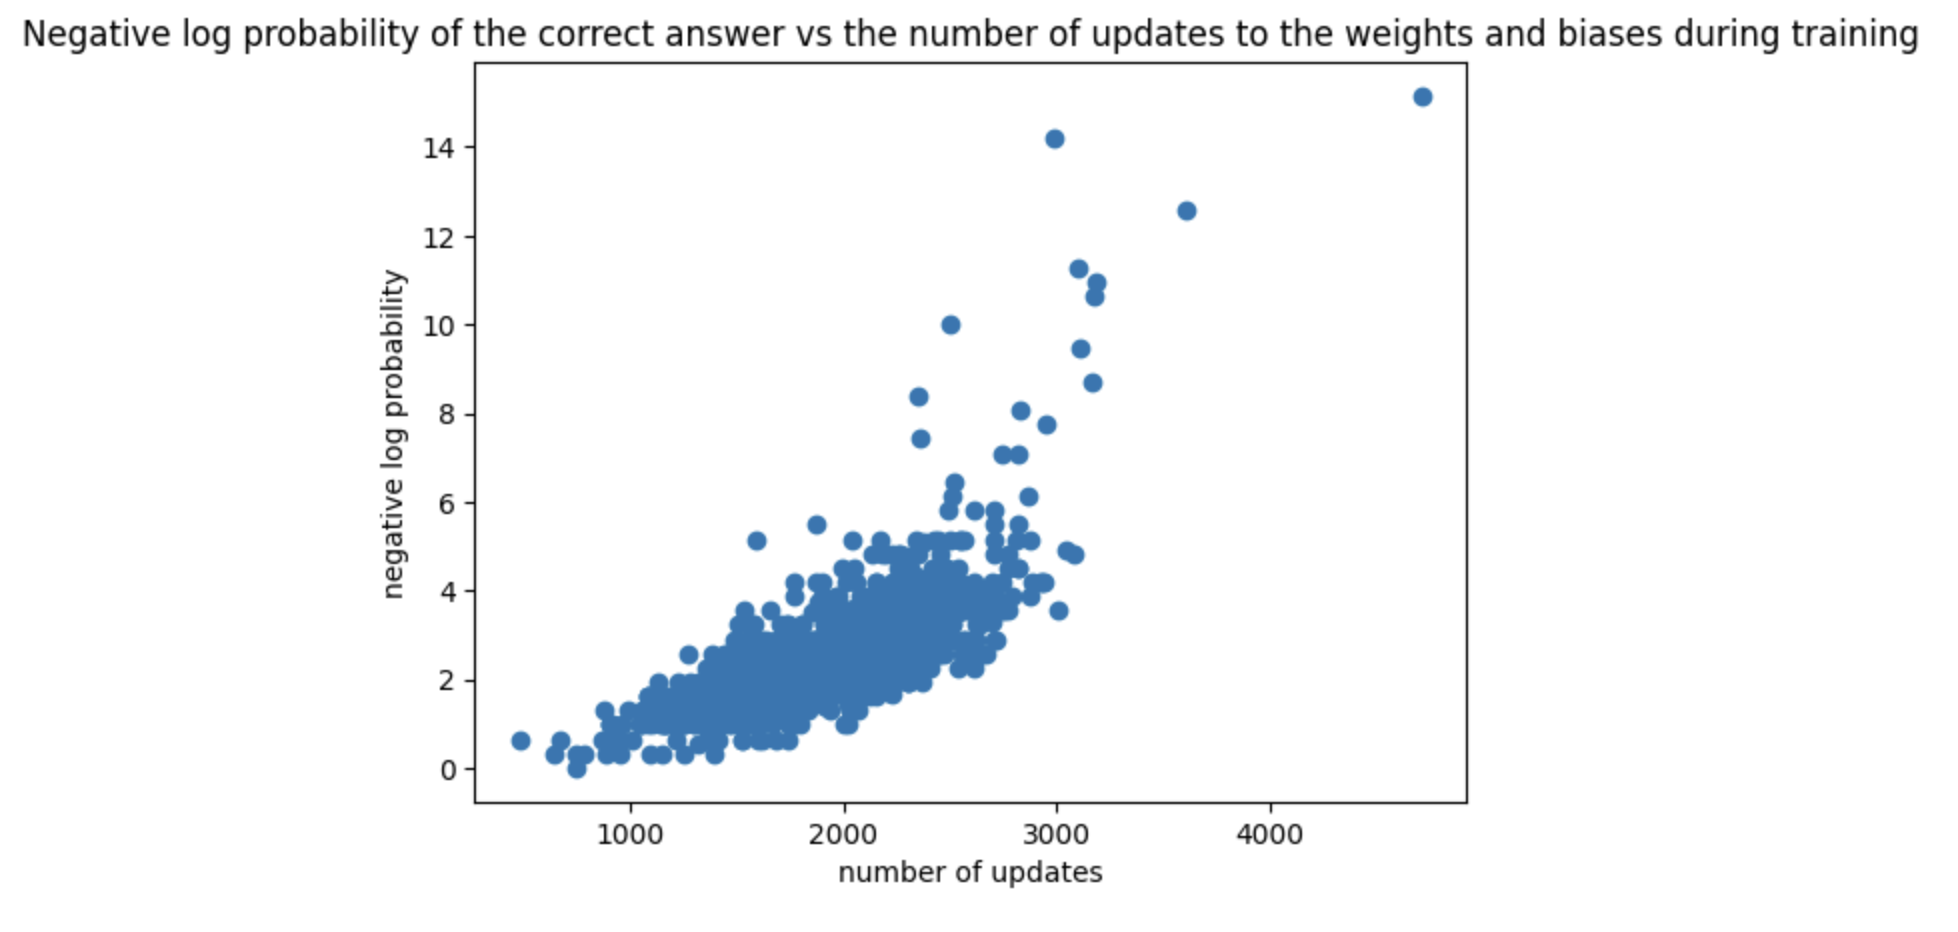
\includegraphics[scale=0.5]{neg-loss-vs-updates.png}
    \caption{Graph of negative loss probability vs the number of updates.}
    \label{fig:randim}
\end{figure*}

The value of the negative log probability is high when the probability for the correct answer is low. Ideally, we want to update the weights more frequently when the neural network is not performing well. This is illustrated in the graph above. As the negative log probability of the correct answer increased, so did the number of updates to the weights.

\begin{figure*}[h!]
    \centering
    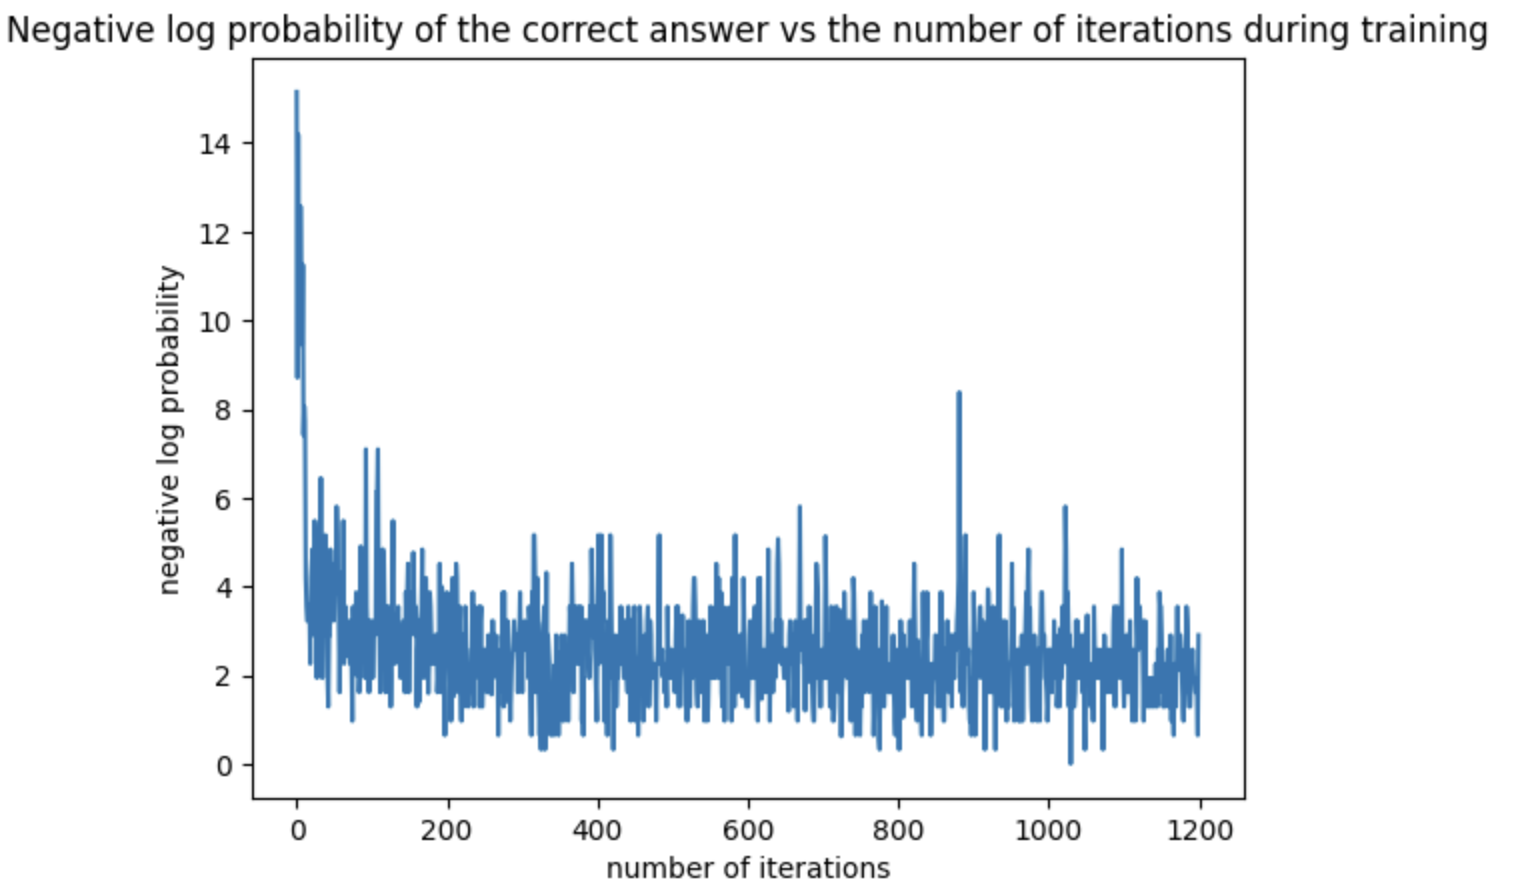
\includegraphics[scale=0.5]{neg-loss-vs-iterations.png}
    \caption{Graph of negative loss probability vs the number of iterations.}
    \label{fig:randim}
\end{figure*}

The performance of a neural network improves during training. At first, it performs poorly because its weights were randomly initialized. As more batches of images are fed to the neural network, it begins predicting the correct answer with higher probabilities. This is illustrated in the graph above. As the number of iterations increased (i.e the number of batches fed to the model), the negative log probability of the correct answer decreased because the model was improving. \\\\
\begin{figure*}[h!]
    \centering
    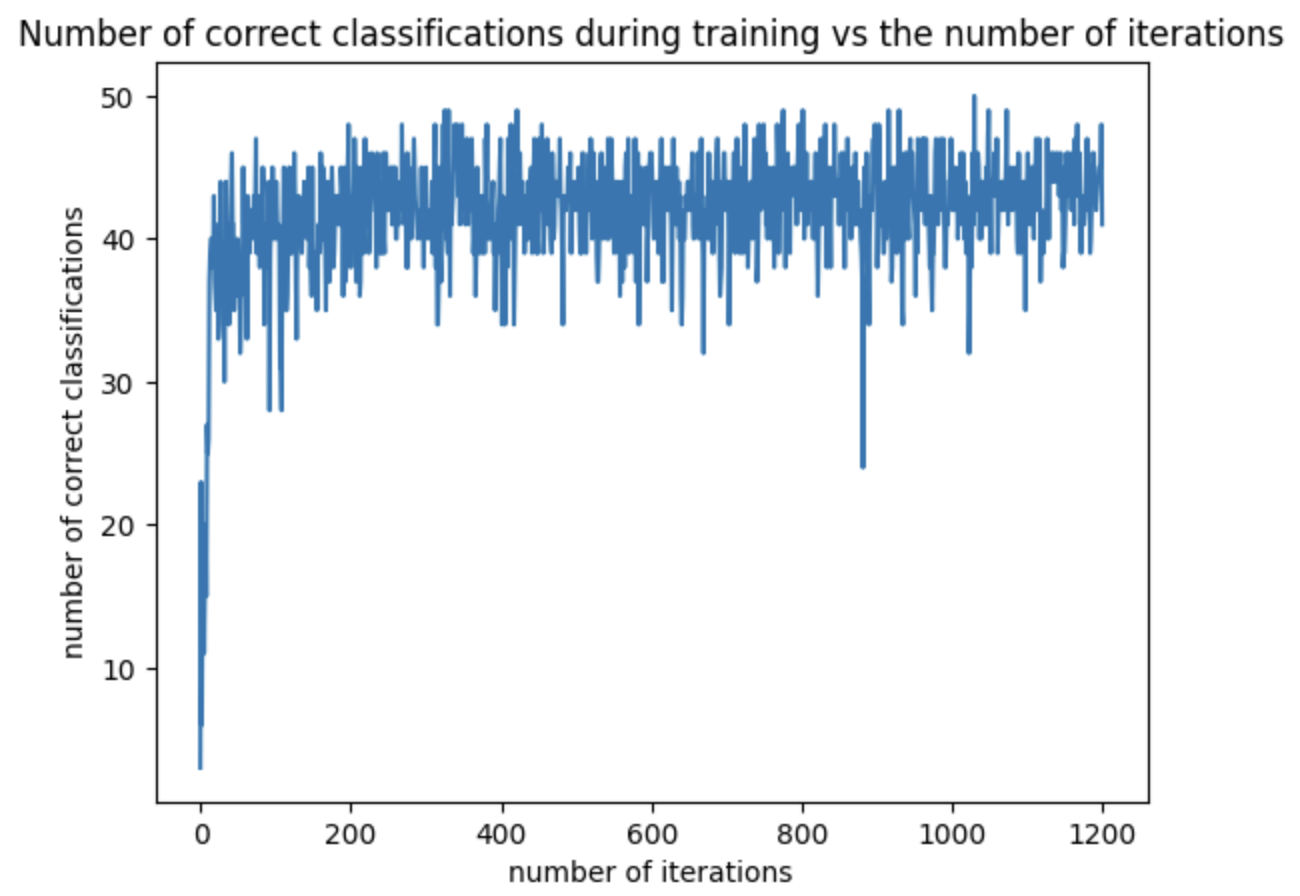
\includegraphics[scale=0.5]{classifications-vs-iterations-training.png}
    \caption{Graph of number of correct classifications vs number of iterations during training.}
    \label{fig:randim}
\end{figure*}
One way of measuring the performance of the model during training is by looking at the accuracy of each batch. The accuracy is defined as the total number of correct classifications divided by the size of the batch. At first, the model was performing very poorly because the weights were randomly initialized. For instance during the first couple of iterations, only about 10 images out of 50 were correctly classified. As the number of iterations increased, so did the number of correct classifications because the model was learning.

\begin{figure*}[h!]
    \centering
    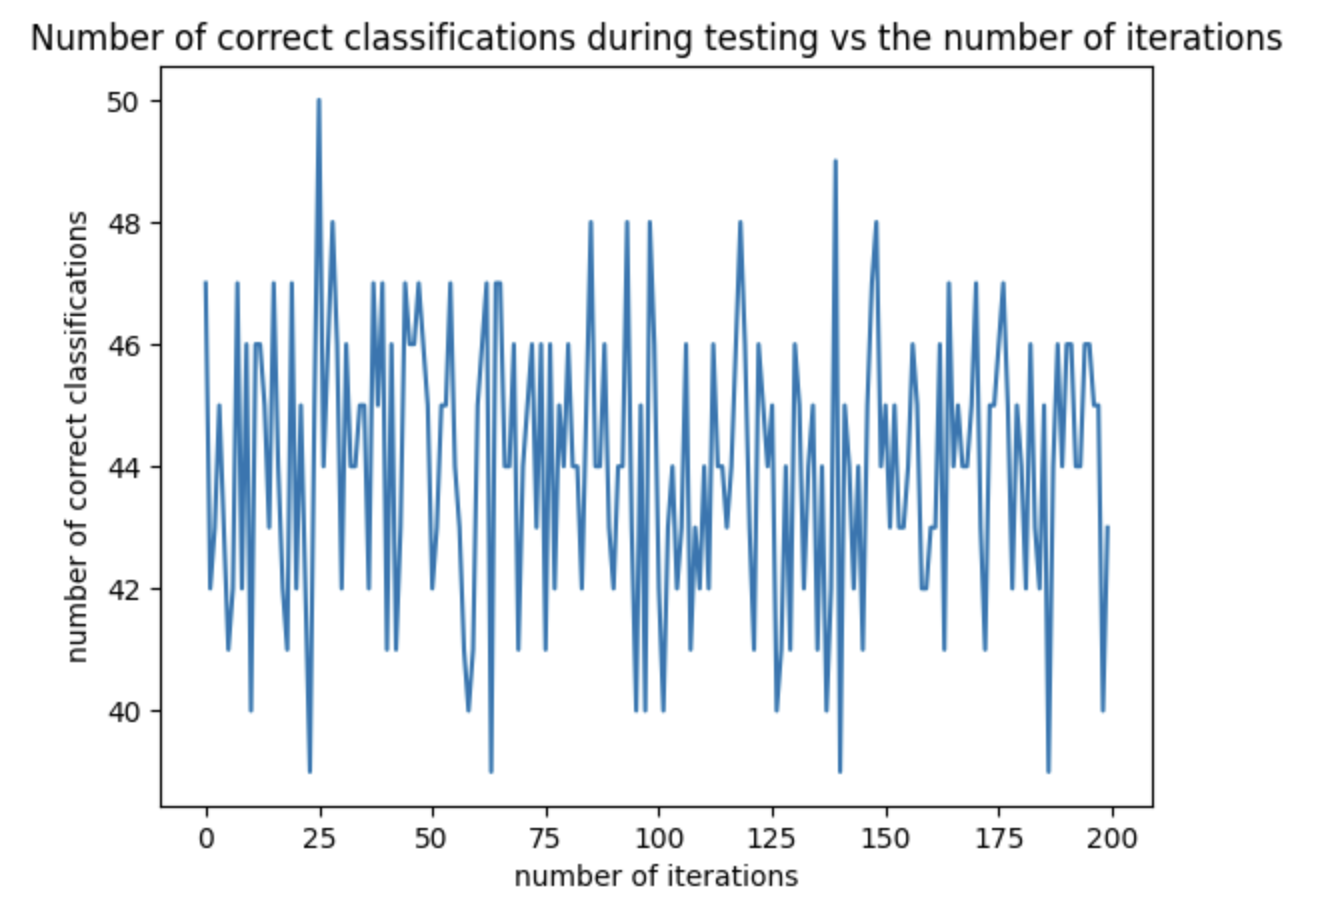
\includegraphics[scale=0.5]{classifications-vs-iterations-test.png}
    \caption{Graph of number of correct classifications vs number of iterations during tesing.}
    \label{fig:randim}
\end{figure*}
The performance of a trained neural network is evaluated using the testing dataset. The model performs quite well, giving an average accuracy of about 90 \% across all the batches. As the graph shows, roughly 45 images out of 50 are correctly classified across all the batches. \\

The overall accuracy of the testing data was equal to 90.07 \%
\end{homeworkProblem}
\clearpage

%----------------------------------------------------------------------------------------
%	PROBLEM 6
%----------------------------------------------------------------------------------------

\begin{homeworkProblem}
In this section, we attempt to visualize what the network is doing by visualizing the weights as if they were digits. Each of the 10 output neurons has 784 inputs and thus 784 weights. We visualize the weights of the output neurons by plotting the following heatmap.

\begin{figure*}[h!]
    \centering
    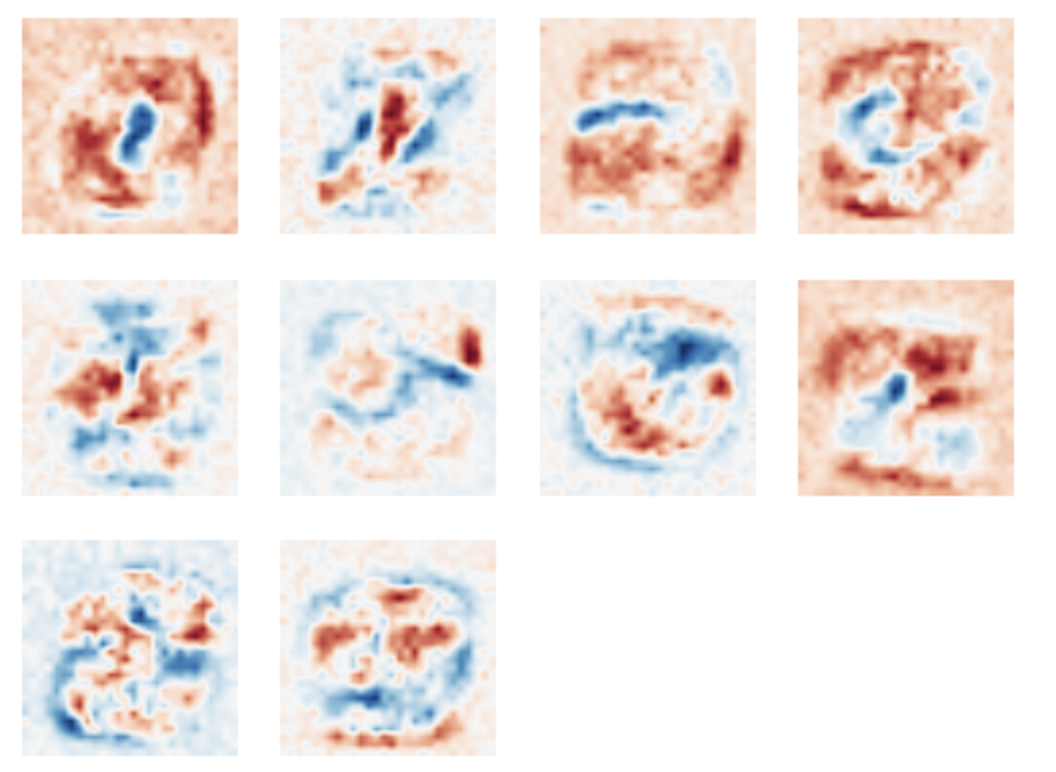
\includegraphics[scale=0.5]{heatmap.png}
    \caption{Heatmap of weights of output neurons}
    \label{fig:randim}
\end{figure*}
The weights corresponding to the output neuron which classifies digits as 3 has the shape of the digit 3. This is also the case for digit 0, 2 and 7. The digits formed on the  other heatmaps are less discernible.
It seems that the weights take the shape of the digit they are predicting.
\end{homeworkProblem}
\clearpage

%----------------------------------------------------------------------------------------
%	PROBLEM 7
%----------------------------------------------------------------------------------------

\begin{homeworkProblem}
We will now use a high-level library to implement a Neural Network. We use the the Keras Module from the Tensor Flow library to implement the model. The design of the model is in the figure below. 
\begin{figure*}[h!]
    \centering
    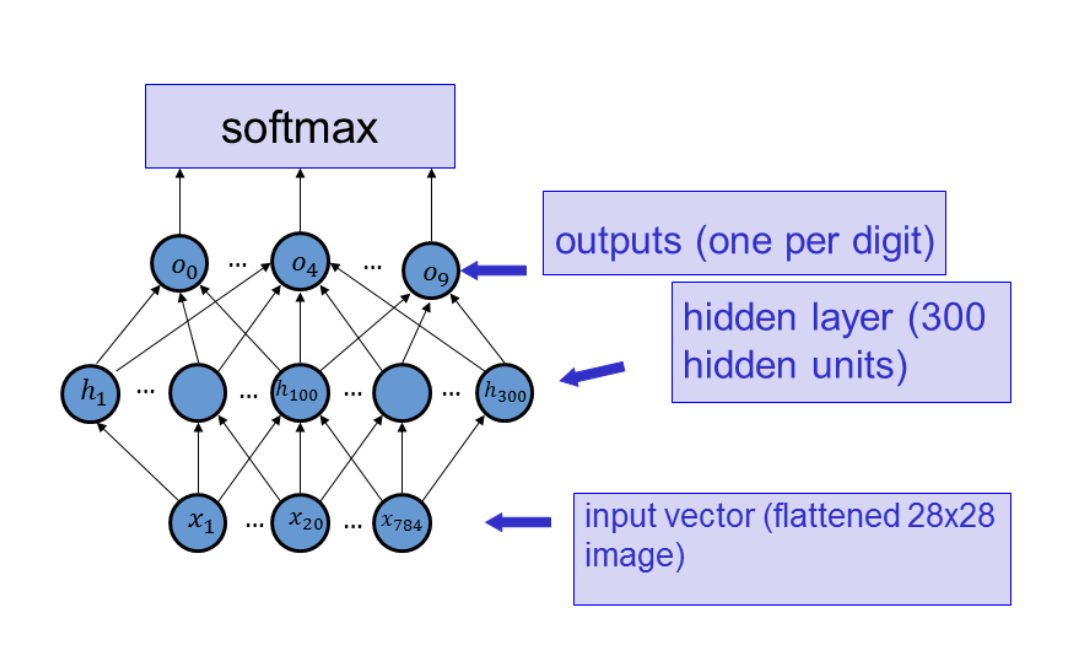
\includegraphics[scale=0.25]{Network Diagram.png}
    \caption{Diagram of the layers for the Neural Network in Keras.}
    \label{fig:randim}
\end{figure*}
We were also instructed have a tanh activation function between the hidden layer and the out layer of our network. We first have to preprocess our data by normalizing our values then reshape our data such taht each entry in our dataset is (28, 28) NumPy array. We create a model object with object with an array parameter defining our model's layer.
\begin{lstlisting}[language=Python]
model = tf.keras.models.Sequential([
  tf.keras.layers.Flatten(input_shape=(28, 28)),
  tf.keras.layers.Dense(300, activation='tanh'),
  tf.keras.layers.Dense(10, activation='softmax')
])
\end{lstlisting}
The parameter defining our network is an array with the layers that we would incorporate into our model. The first layer is 784 neuron and takes in a 2 Dimensional NumPy array and flattens the data. The second layer is a hidden layer with 300 neuron with tanh activation function, and the third layer is the output layer which categories the letters with softmax activation function.

We now compile our model using the adam optimization algorithm with a learning rate of 0.001 and with with Keras cross entropy loss function for sparsely populated vector for best result. We also measure correct classification with Keras category Accuracy metric for sparsely populated vectors. 


\end{homeworkProblem}
\clearpage


%----------------------------------------------------------------------------------------
%	PROBLEM 8
%----------------------------------------------------------------------------------------
%using mini-batch gradient descent, using the training set provided to you. You should be able to obtain test
%classification performance of over 95 percent correct classification. A learning rate of about 0.01 and batch sizes of 50 should work well.
%For the training and the test set, graph the correct answer cost function and correct classification rate versus the number of updates to
%the weights and biases during training. (I.e., plot the learning curves.)
%In your report, display 20 digits which were classified correctly, and 10 digits from the test set which were classified incorrectly.

\begin{homeworkProblem}
We fit the model using the training data and set our batch size hyperparameter to be 50 in order to perform mini-batch gradient descent. We also give our testing data as a validation set in Keras to see how our model performs with the testing data as we are fitting our data. We also set our epoch hyperparameter to be 6 such that keras will go through 6 passes on our dataset for fitting the model to the training dataset.  The resulting model will give us an accuracy of 97\% on our testing set. \\

We now plot the Correct Answer Loss function and Correct Classification Rate versus number of updates to the weights and biases. We use the keras model history object to obtain the history of our loss function during the fitting process and since we added an accuracy metric to the model, we also obtain the classification rate of our model. Keras updates the weights and biases of the model every epoch which leads thus our x-axis will be epoch value during training.  We see the 2 plots in the figure below. 

\begin{figure*}[h!]
    \centering
    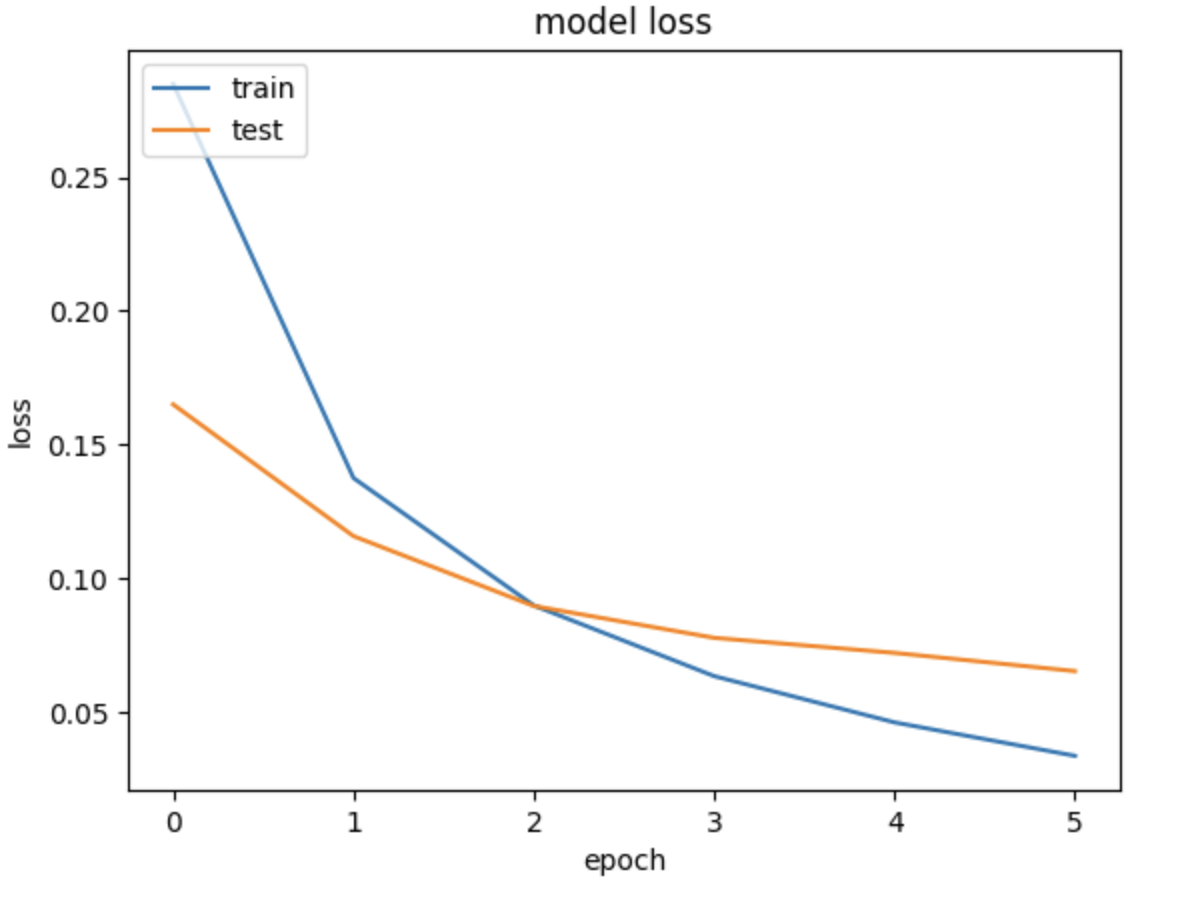
\includegraphics[scale=0.5]{keras-model-loss.png}
    \caption{Graph of the model loss vs the number of epochs.}
    \label{fig:randim}
\end{figure*}

The loss decreases as the number of epochs increases. This is because with each epoch, the weights of the model are updated in such a way that the model is able to make better predictions. This will result in fewer misclassifications which will cause the loss to decrease.


\begin{figure*}[h!]
    \centering
    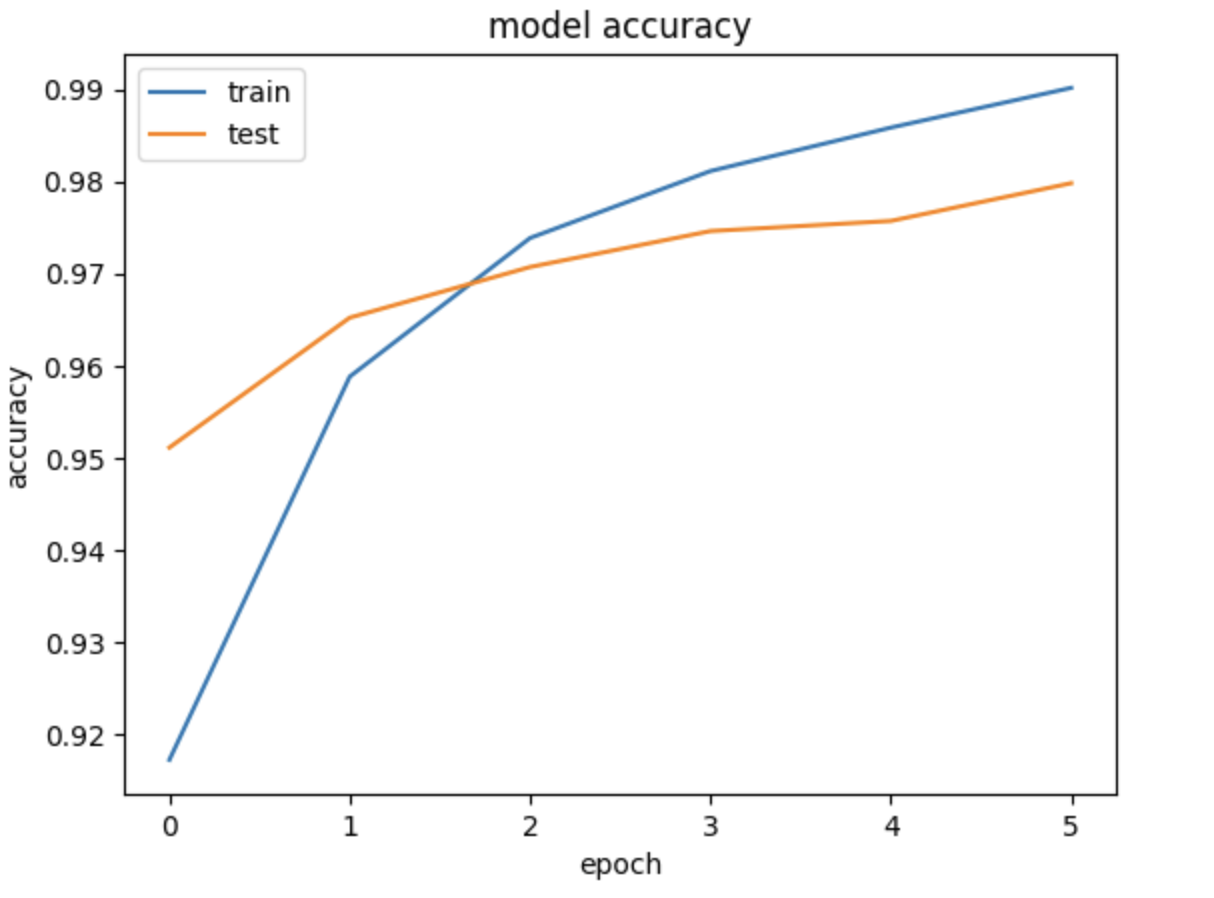
\includegraphics[scale=0.5]{keras-model-accuracy.png}
    \caption{Graph of the model accuracy vs the number of epochs..}
    \label{fig:randim}
\end{figure*}

As the number of epochs increases, so does the accuracy. This is because with each epoch, the weights of the model are updated in such a way that the model is able to make better predictions.


\end{homeworkProblem}
\clearpage

%----------------------------------------------------------------------------------------
%	PROBLEM 9
%----------------------------------------------------------------------------------------

\begin{homeworkProblem}
In this section, we attempt to visualize what the network is doing by visualizing the weights connected to the hidden layer as if they were digits. We select 2 interesting set of weights to visualize based on the following criterion: For example, for the output neuron 2, we found all of the 300 weights connected to that output neuron and determined the highest weight. The highest weight was coming from the 92nd neuron in the hidden layer. We then visualized the 784 weights connected to that neuron in the hidden layer. The following image is the heatmap obtained by visualizing these weights:

\begin{figure*}[h!]
    \centering
    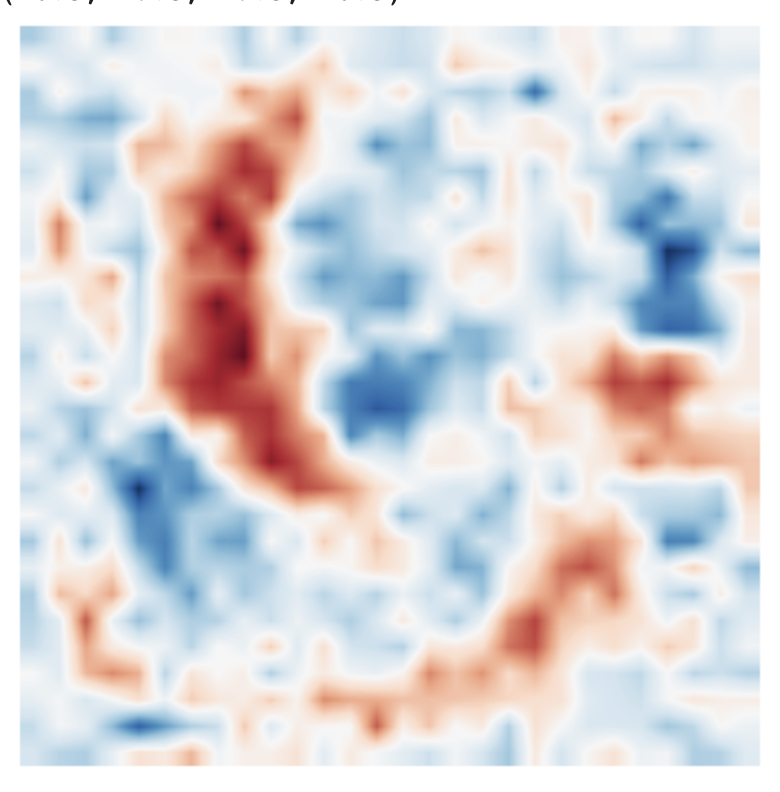
\includegraphics[scale=0.25]{hidden-neuron-91.png}
    \caption{Heatmap obtained from the weights of the 92nd neuron in the hidden layer.}
    \label{fig:randim}
\end{figure*}

It seems that the weights have the shape of the digit 2. It is accomplishing edge detection for 2.\\

We repeated the same process for the output neuron 3 and got the following heatmap:

\begin{figure*}[h!]
    \centering
    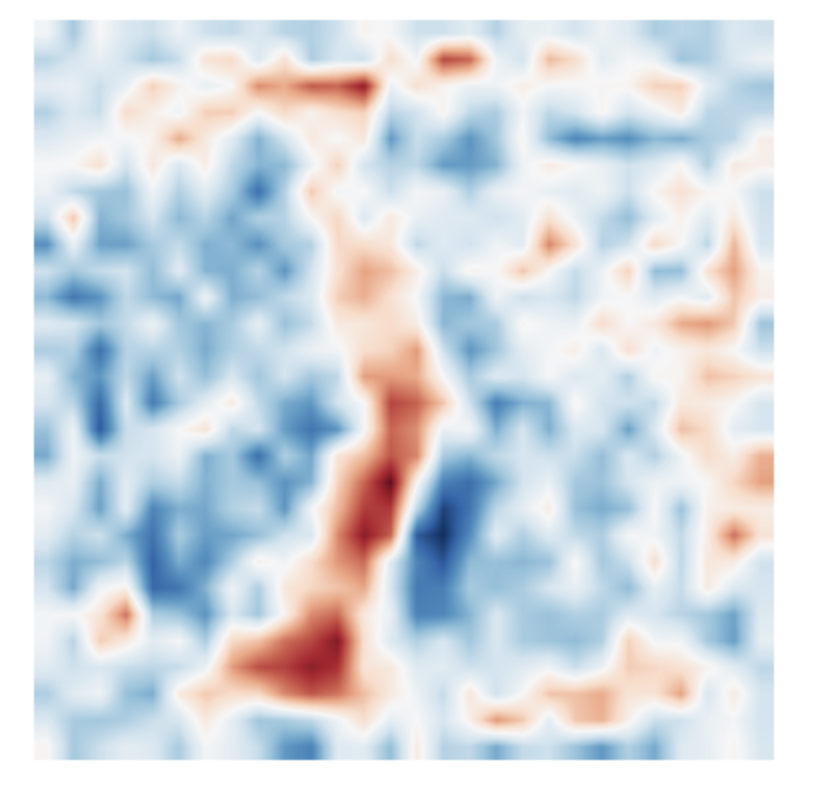
\includegraphics[scale=0.25]{hidden-neuron-186.png}
    \caption{Heatmap obtained from the weights of the 187th neuron in the hidden layer.}
    \label{fig:randim}
\end{figure*}

It seems that the weights have the shape of the digit 3.
\end{homeworkProblem}
\clearpage

\end{document}